\documentclass[runningheads,14pt,a4paper,openany]{book}

% Добавя възможност за сензитивни хипер-връзки в самия документ.
\usepackage[linktocpage=true,bookmarks=false]{hyperref}
\usepackage{nameref}
\usepackage[utf8x]{inputenc}
\usepackage[english,bulgarian]{babel}
\usepackage{url}
\usepackage{lipsum}
% Според изискванията на ИИКТ-БАН не бива да има номерация на страниците в ръкописа.
%\usepackage{nopageno}
\usepackage{shorttoc}
\usepackage[pdftex]{graphicx}
% Директория в която се намират изображенията.
\graphicspath{{images/}}
\usepackage{array,arydshln}
\usepackage{imakeidx}
\usepackage{placeins}
% Използва се за включване на кориците под формата на PDF файлове.
\usepackage{pdfpages}
% Служи за управление на заглавията.
\usepackage{fancyheadings}
%\usepackage{bookmark}

% Добавени от доц. Вера Ангелова.
%\usepackage{amsmath,amssymb,amsthm}
%\usepackage{longtable}
%\usepackage{pifont}   
%\usepackage{epsfig}
%\usepackage{tocloft}
%\usepackage{etoc}
%\usepackage{wasysym}
%\usepackage{eurosym}
%\usepackage{slashbox}
%\usepackage{soul}
%\usepackage{enumitem}
%\usepackage{mathcomp}
%\usepackage{epstopdf}
%\usepackage{latexsym}
%\usepackage{eucal}
%\usepackage{mathrsfs}

\textheight 22.8cm
\textwidth 17cm
\oddsidemargin -0.54cm
\evensidemargin -0.54cm
\topmargin 1.5cm

\parskip=0.2cm
\parindent=20pt
\flushbottom

% Премахва подчертаващата линия в заглавните части.
\renewcommand{\headrulewidth}{0pt}

\selectlanguage{bulgarian}

\lhead[\thepage \quad Тодор Балабанов \quad \hfill]{}
\chead{}
\rhead[]{\hfill Apache OpenOffice Calc за корпоративна употреба \quad \thepage }
\lfoot{}
\cfoot[\em Лекции по компютърни науки и технологии на ИИКТ - БАН, № *, 20**]{\em Лекции по компютърни науки и технологии на ИИКТ - БАН, № *, 20**} 
\rfoot{}

\onecolumn
\makeindex[columns=1, title=Азбучен указател, intoc]

\begin{document}

\def\ql{\textquotedblleft}\def\qr{\textquotedblright}


\includepdf[pages={1,2}]{images/front}
\thispagestyle{empty}

\voffset =-1truecm

% Използва се за номерация на страниците.
\renewcommand{\thepage}{\roman{page}}

\setcounter{page}{-1}
\thispagestyle{empty}
\pagestyle{empty}
\thispagestyle{empty}

% Тук стои таблицата със съдържанието, което се генерира от названието на главите.
\newpage
\thispagestyle{empty}
\pagestyle{empty}
\shorttoc{Теми}{0}
\thispagestyle{empty}
\pagestyle{empty}

% Тук стои таблицата със съдържанието, което се генерира от названието на главите и названието на секциите в тях.
\newpage
\thispagestyle{empty}
\pagestyle{empty}
\thispagestyle{empty}
\tableofcontents
\thispagestyle{empty}
\pagestyle{empty}

% Списък с фигурите.
\newpage
\listoffigures
\addcontentsline{toc}{chapter}{Списък на фигурите}

% Списък с таблиците. 
\newpage
\listoftables
\addcontentsline{toc}{chapter}{Списък с таблиците}

\newpage
\addcontentsline{toc}{chapter}{Предговор}
\chapter*{Предговор}
\pagenumbering{arabic}
\setcounter{page}{1}
\pagestyle{fancyplain}

Calc е софтуер за електронни таблици, който влиза в състава на програмния продукт Apache OpenOffice. По настояще Calc се разпространява като софтуер с отворен код под два основни лиценза – SISSL и GNU LGPL. Calc основно се използва за създаване и оформление на таблици, изчисления, обработка и анализ на данни, както и за графично представяне на резултатите от обработката. Учебното помагало е предназначено за офис работници (ръководители, мениджъри, секретари, финансови анализатори и други), ученици и студенти. 

Учебното помагало представя графичния интерфейс на Calc. Демонстрирате се основните елементи на потребителския интерфейс и начина за работа с тях. Засягат се темите за работа с файловата система на операционната система. Отделя се внимание за начина по който Calc зарежда и съхранява файлове, както и за възможностите да обработва информация от алтернативни софтуерни продукти за електронни таблици. Засягат се въпросите за работа с документи и списъчна информация. Набляга се на въвеждането, манипулирането и обработването на таблична информация. Значително внимание се отделя на възможностите за изчисления в Calc. Акцент е работата с формули, организиране на изчисленията и използването на наличните в Calc математически функции. Допълнително внимание е отделено за форматирането на таблиците и графичното им оформление. Разглеждат се възможностите за сортиране и филтриране на данни. Демонстрират се основни принципи за защита на информацията. Представя се работа с диаграми от различни видове – създаване, редакция, оформление и настройки. Засягат се темите за оформление на печатните страници и разпечатването на принтер. 

Глава 1 - \nameref{chapter01}: Представя процеса по изтегляне, инсталиране и стартиране на програмния продукт.

Глава 2 - \nameref{chapter02}: Запознава с основните елементи на графичния потребителски интерфейс в основния работен прозорец.


\newpage
\chapter{Инсталация и стартиране}
\label{chapter01}

\newpage
\addcontentsline{toc}{chapter}{Заключение}
\chapter*{Заключение}


% Списък с използвана литература и източници на информация.
\newpage
\begin{thebibliography}{99}
\addcontentsline{toc}{chapter}{Библиография}
\end{thebibliography}

% Азбучен указател на използваните термини.
\newpage
\printindex

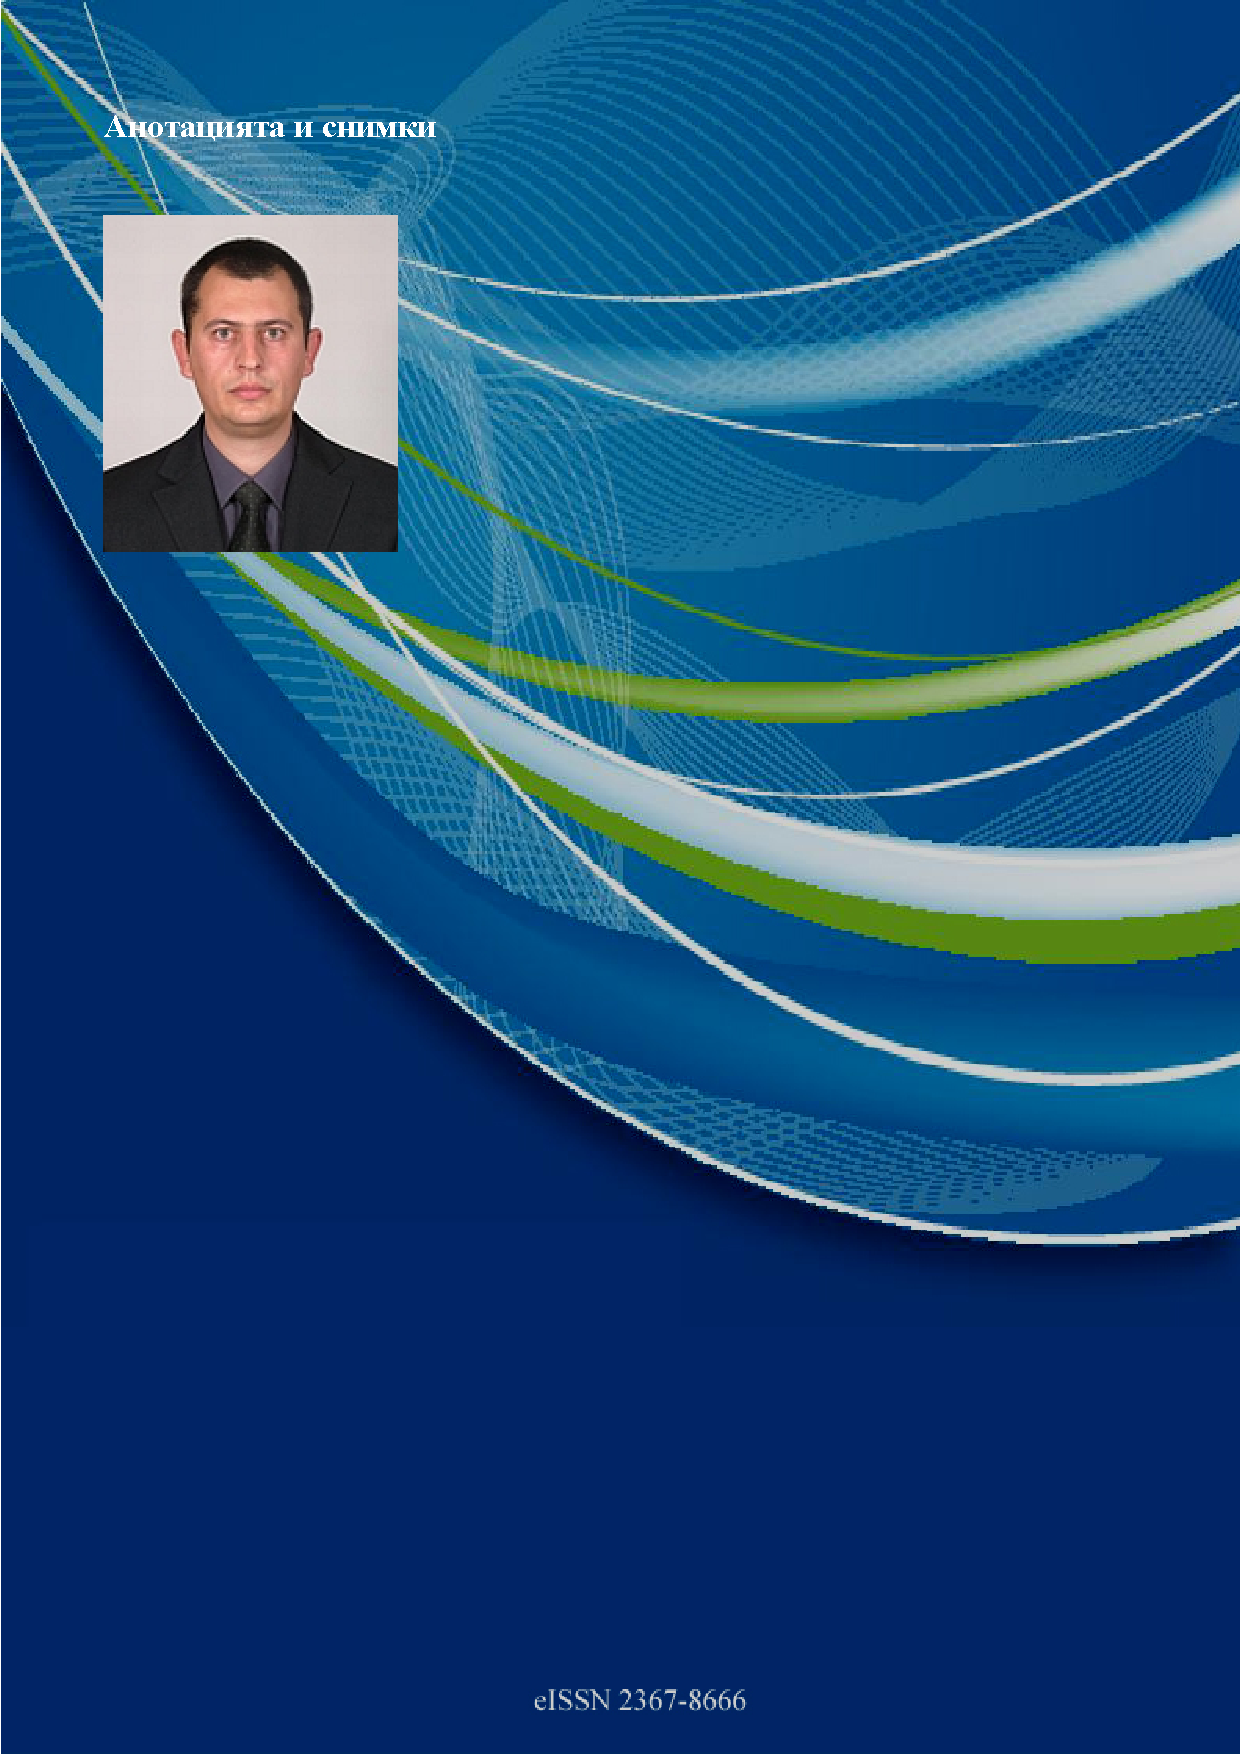
\includepdf[pages=-,height=320mm]{images/back}
\end{document}
